\documentclass[../main.tex]{subfiles}
\graphicspath{{\subfix{../Images/}}}

\begin{document}

\chapter*{Plates}

\FloatBarrier
\begin{figure}
    \centering
    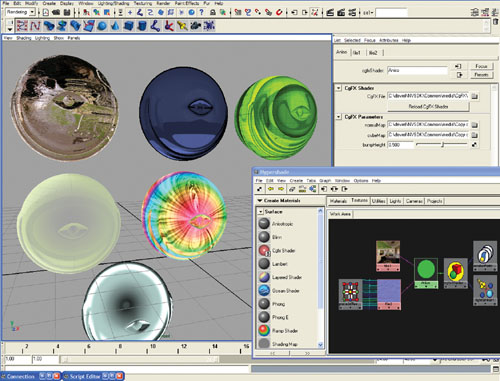
\includegraphics[width=1\linewidth]{plate_1.jpg}
    \caption{Plate 1 Cg Shaders in Maya 4.5 Using the Maya Cg Plug-in}
    \label{fig:plate-1}
\end{figure}
\FloatBarrier
\begin{figure}
    \centering
    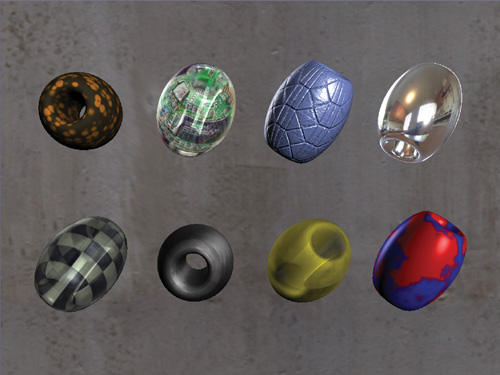
\includegraphics[width=1\linewidth]{plate_2.jpg}
    \caption{Plate 2 Bead Shapes Rendered with Maya and Cg on the NVIDIA Quadro FX}
    \label{fig:plate-2}
\end{figure}
\FloatBarrier
\begin{figure}
    \centering
    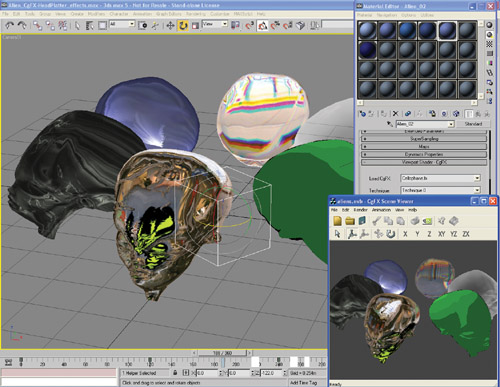
\includegraphics[width=1\linewidth]{plate_3.jpg}
    \caption{Plate 3 Discreet 3ds max 5 and the 3ds max Cg Plug-in}
    \label{fig:plate-3}
\end{figure}
\FloatBarrier
\begin{figure}
    \centering
    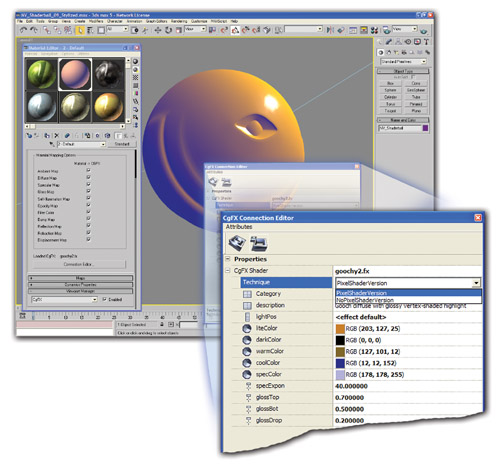
\includegraphics[width=1\linewidth]{plate_4.jpg}
    \caption{Plate 4 The 3ds max Cg Plug-in and Connection }
    \label{fig:plate-4}
\end{figure}
\FloatBarrier
\begin{figure}
    \centering
    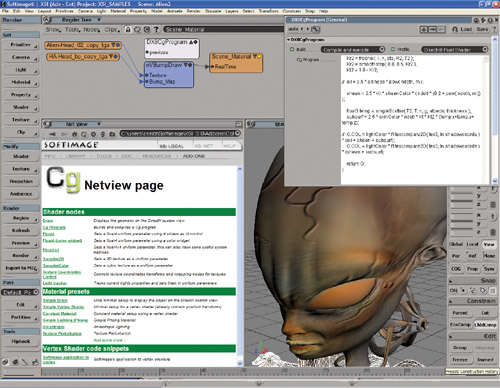
\includegraphics[width=1\linewidth]{plate_5.jpg}
    \caption{Plate 5 Softimage|XSI v.3.0 Integrating Cg}
    \label{fig:plate-5}
\end{figure}
\FloatBarrier
\begin{figure}
    \centering
    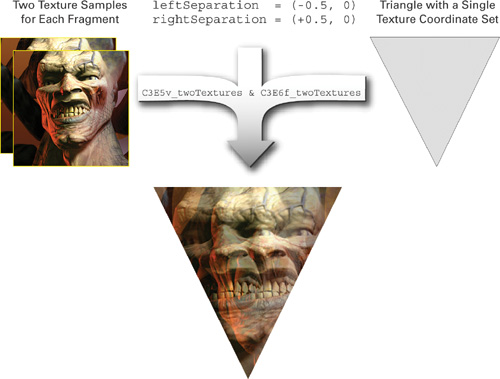
\includegraphics[width=1\linewidth]{plate_6.jpg}
    \caption{Plate 6 Creating a Double Vision Effect}
    \label{fig:plate-6}
\end{figure}
\FloatBarrier
\begin{figure}
    \centering
    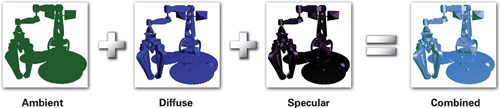
\includegraphics[width=1\linewidth]{plate_7.jpg}
    \caption{Plate 7 Combining the Ambient, Diffuse, and Specular Lighting Terms}
    \label{fig:plate-7}
\end{figure}
\FloatBarrier
\begin{figure}
    \centering
    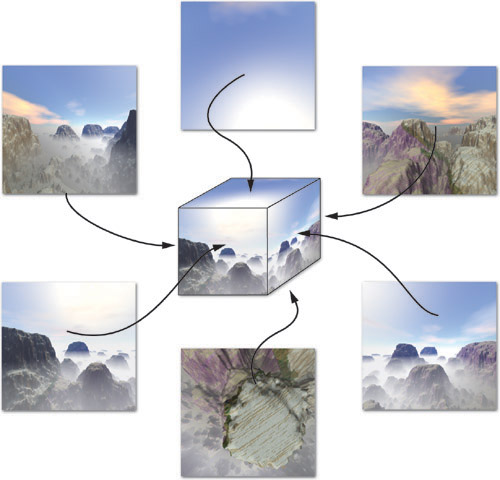
\includegraphics[width=1\linewidth]{plate_8.jpg}
    \caption{Plate 8 Six Texture Images Combined to Form a Cube Map}
    \label{fig:plate-8}
\end{figure}
\FloatBarrier
\begin{figure}
    \centering
    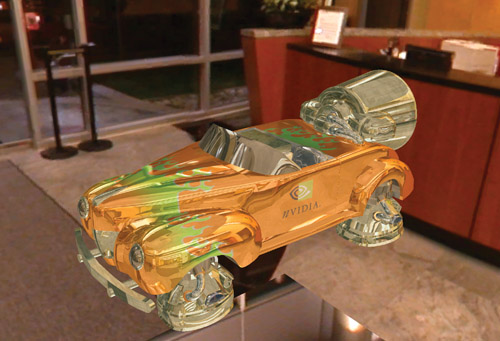
\includegraphics[width=1\linewidth]{plate_9.jpg}
    \caption{Plate 9 Reflective Environment Mapping}
    \label{fig:plate-9}
\end{figure}
\FloatBarrier
\begin{figure}
    \centering
    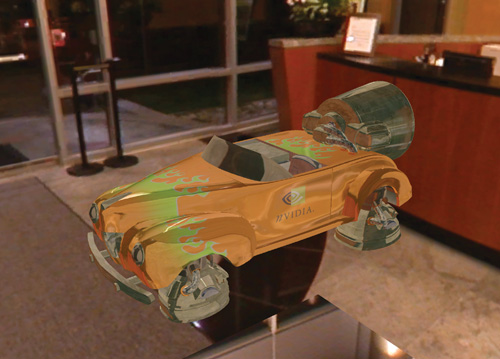
\includegraphics[width=1\linewidth]{plate_10.jpg}
    \caption{Plate 10 Refractive Environment Mapping}
    \label{fig:plate-10}
\end{figure}
\FloatBarrier
\begin{figure}
    \centering
    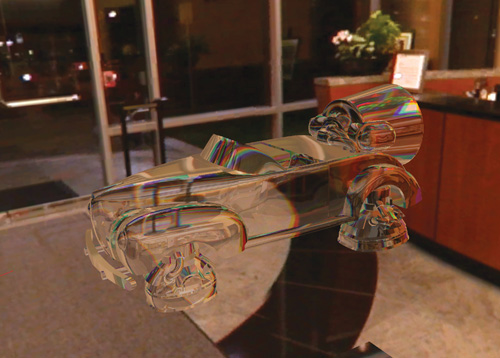
\includegraphics[width=1\linewidth]{plate_11.jpg}
    \caption{Plate 11 The Fresnel Effect and Chromatic Dispersion}
    \label{fig:plate-11}
\end{figure}
\FloatBarrier
\begin{figure}
    \centering
    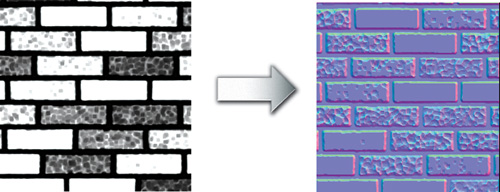
\includegraphics[width=1\linewidth]{plate_12.jpg}
    \caption{Plate 12 A Grayscale Height Field Converted to a Range-Compressed Normal Map}
    \label{fig:plate-12}
\end{figure}
\FloatBarrier
\begin{figure}
    \centering
    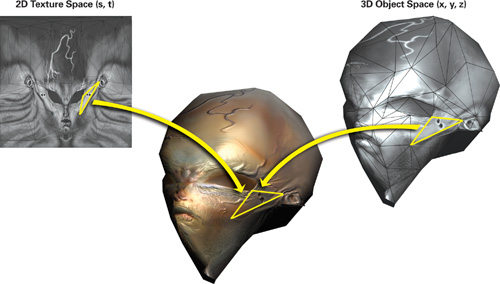
\includegraphics[width=1\linewidth]{plate_13.jpg}
    \caption{Plate 13 Bump Mapping a Textured Polygonal Mesh}
    \label{fig:plate-13}
\end{figure}
\FloatBarrier
\begin{figure}
    \centering
    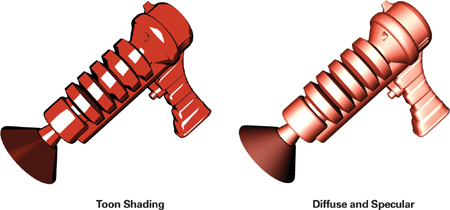
\includegraphics[width=1\linewidth]{plate_14.jpg}
    \caption{Plate 14 Nonphotorealistic Rendering}
    \label{fig:plate-14}
\end{figure}
\FloatBarrier
\begin{figure}
    \centering
    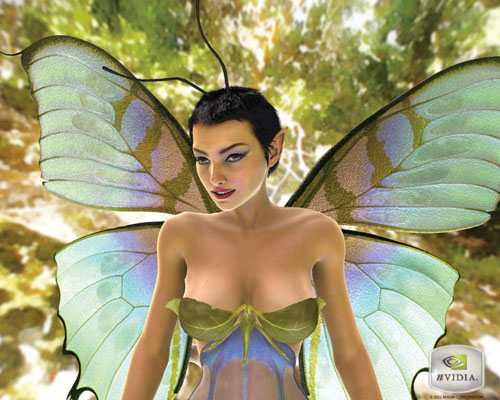
\includegraphics[width=1\linewidth]{plate_15.jpg}
    \caption{Plate 15 The Dawn Character, Driven by Shaders for the Skin's Surface, Skeletal Skinning, and Shape Blending}
    \label{fig:plate-15}
\end{figure}
\FloatBarrier
\begin{figure}
    \centering
    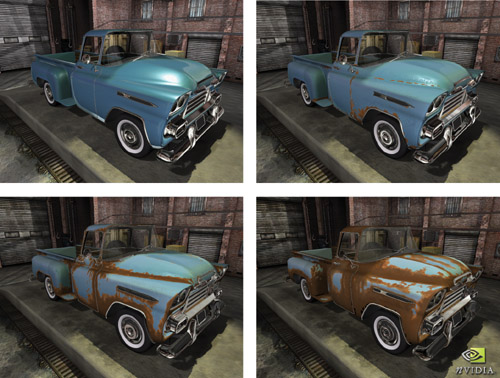
\includegraphics[width=1\linewidth]{plate_16.jpg}
    \caption{Plate 16 NVIDIA Time Machine Demo}
    \label{fig:plate-16}
\end{figure}
\FloatBarrier
\begin{figure}
    \centering
    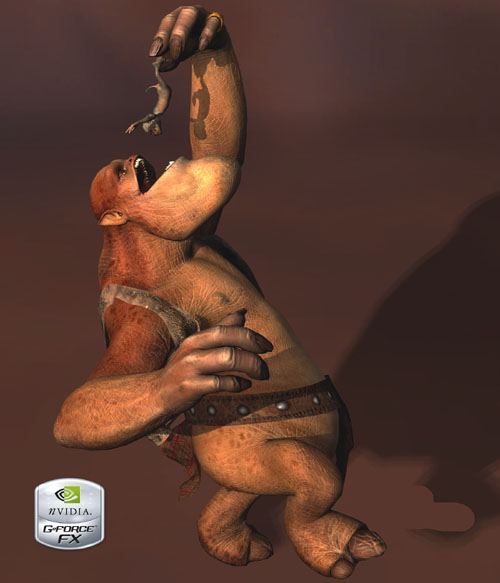
\includegraphics[width=1\linewidth]{plate_17.jpg}
    \caption{Plate 17 NVIDIA Dancing Ogre Demo}
    \label{fig:plate-17}
\end{figure}
\FloatBarrier
\begin{figure}
    \centering
    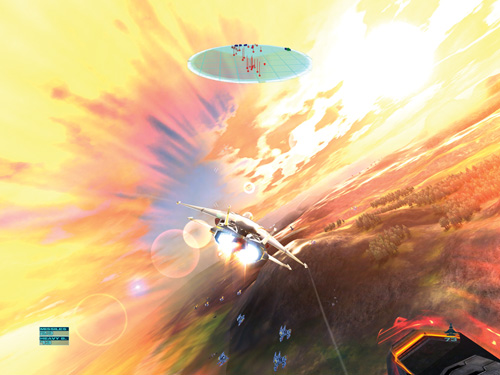
\includegraphics[width=1\linewidth]{plate_18.jpg}
    \caption{Plate 18 Yeti's Gun Metal Game, Using Cg for Advanced Visual Effects}
    \label{fig:plate-18}
\end{figure}
\FloatBarrier
\begin{figure}
    \centering
    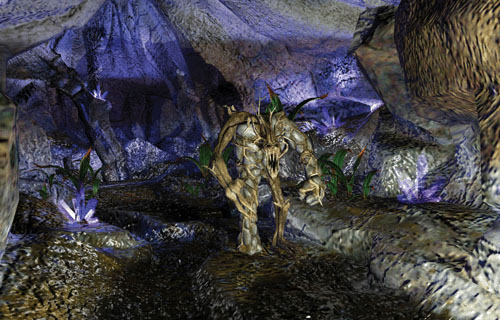
\includegraphics[width=1\linewidth]{plate_19.jpg}
    \caption{Plate 19 Iritor Online, Using Cg Shaders}
    \label{fig:plate-19}
\end{figure}
\FloatBarrier
\begin{figure}
    \centering
    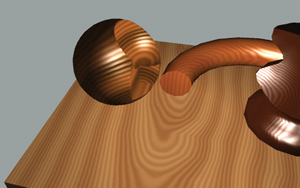
\includegraphics[width=1\linewidth]{plate_20.jpg}
    \caption{Plate 20 Procedural Wood Shader}
    \label{fig:plate-20}
\end{figure}
\FloatBarrier
\begin{figure}
    \centering
    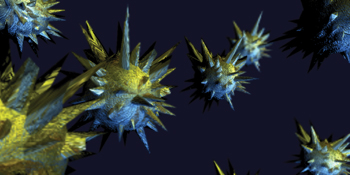
\includegraphics[width=1\linewidth]{plate_21.jpg}
    \caption{Plate 21 Depth of Field}
    \label{fig:plate-21}
\end{figure}
\FloatBarrier
\begin{figure}
    \centering
    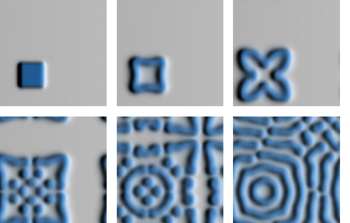
\includegraphics[width=1\linewidth]{plate_22.jpg}
    \caption{Plate 22 Dynamic Reaction Diffusion Textures}
    \label{fig:plate-22}
\end{figure}
\FloatBarrier
\begin{figure}
    \centering
    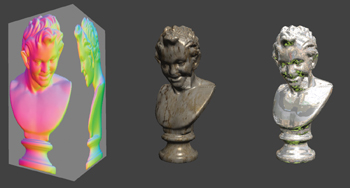
\includegraphics[width=1\linewidth]{plate_23.jpg}
    \caption{Plate 23 Relief Texture Mapping}
    \label{fig:plate-23}
\end{figure}
\FloatBarrier
\begin{figure}
    \centering
    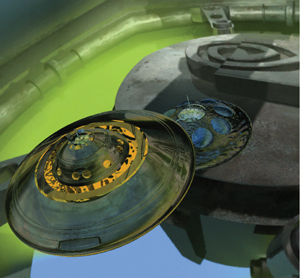
\includegraphics[width=1\linewidth]{plate_24.jpg}
    \caption{Plate 24 Bump Reflection Mapping}
    \label{fig:plate-24}
\end{figure}
\FloatBarrier
\begin{figure}
    \centering
    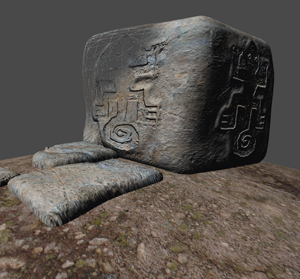
\includegraphics[width=1\linewidth]{plate_25.jpg}
    \caption{Plate 25 Detail Normal Maps}
    \label{fig:plate-25}
\end{figure}
\FloatBarrier
\begin{figure}
    \centering
    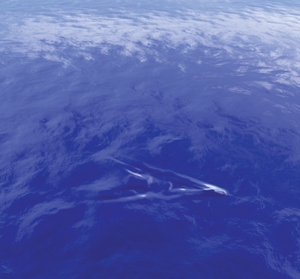
\includegraphics[width=1\linewidth]{plate_26.jpg}
    \caption{Plate 26 Water Interaction}
    \label{fig:plate-26}
\end{figure}
\FloatBarrier
\begin{figure}
    \centering
    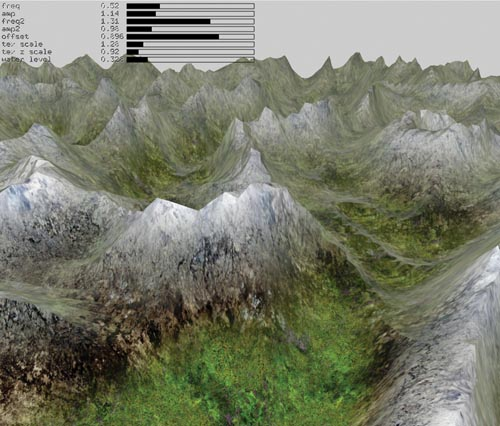
\includegraphics[width=1\linewidth]{plate_27.jpg}
    \caption{Plate 27 A Procedural Terrain Demo}
    \label{fig:plate-27}
\end{figure}
\FloatBarrier
\begin{figure}
    \centering
    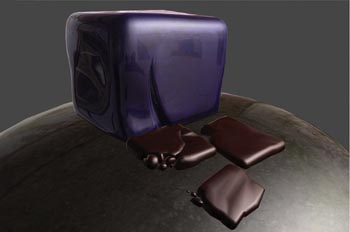
\includegraphics[width=1\linewidth]{plate_28.jpg}
    \caption{Plate 28 Realistic Fresnel Reflection Effects}
    \label{fig:plate-28}
\end{figure}
\FloatBarrier
\begin{figure}
    \centering
    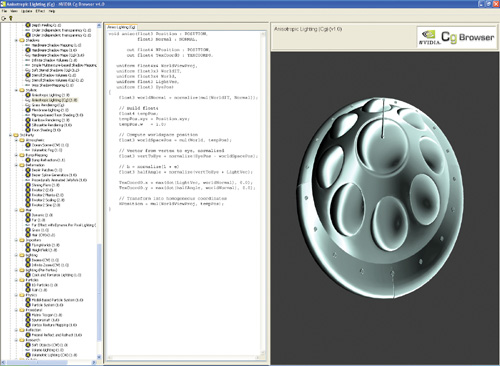
\includegraphics[width=1\linewidth]{plate_29.jpg}
    \caption{Plate 29 The NVIDIA Cg Browser Interface}
    \label{fig:plate-29}
\end{figure}
\FloatBarrier
\begin{figure}
    \centering
    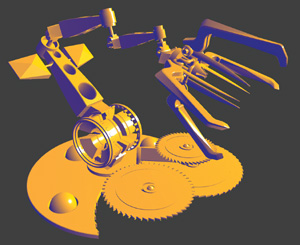
\includegraphics[width=1\linewidth]{plate_30.jpg}
    \caption{Plate 30 A Mechanical Model with a Gooch Cg Shader Applied}
    \label{fig:plate-30}
\end{figure}
\FloatBarrier
\begin{figure}
    \centering
    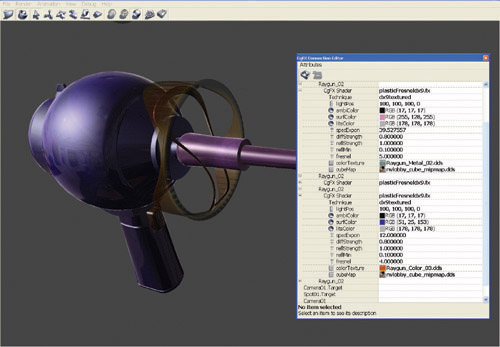
\includegraphics[width=1\linewidth]{plate_31.jpg}
    \caption{Plate 31 Using CgFX to Apply Multiple Shaders to a Ray Gun Model}
    \label{fig:plate-31}
\end{figure}
\FloatBarrier

\end{document}